\chapter{DevOps\label{devops}}

DevOps:illa tarkoitetaan ohjelmistokehityksen (engl. \textit{development}) ja IT-toimintojen (engl. \textit{operations}) yhdistämistä.
DevOps:iin liitetään usein jatkuva integraatio ja toimitus sekä automaatio ja laadunvalvonta \cite{Jabbari16}.
DevOps:ia käsitteenä voidaan tarkastella ajattelutapana tai käytännön ohjelmistotuotannon toimintamallinna.

DevOps ajattelutapana pyrkii ohjelmistokehityksen ja IT-toimintojen jaon välttämiseen ja yhteistoiminnan mahdollistavan kulttuurin rakentamiseen \cite{Klein21}.
DevOps toimintamallina taas keskittyy käytännön toimiin ja teknologioihin, jotka mahdollistavat DevOps-ajattelutavan mukaisen ohjelmistotuotannon.
Tässä tutkielmassa keskitytään aiheen käsittelyyn käytännön toimintamallin kautta.

\section{DevOps-toimintamalli}

DevOps-toimintamalli painottaa jatkuvaa integraatiota ja toimitusta (CI/CD) sekä laadunvalvontaa käyttäen standardisoituja automaattisia menetelmiä. Kuva~\ref{fig:devops} visualisoi DevOps-toimintamallin eri vaiheita. Kehitys- ja operaatiovaiheet tapahtuvat limittäin ja koko prosessi voidaan suorittaa useita kertoja päivässä automatisoidun julkaisuputken avulla. \cite{Jabbari16}

\begin{figure}[ht]
\begin{center}
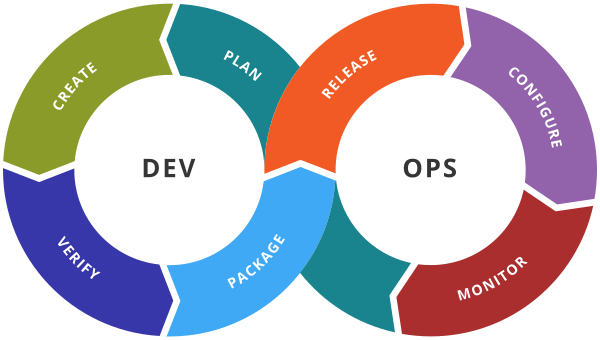
\includegraphics[width=0.6\textwidth]{figures/devops_toolchain.png}
\caption{DevOps-toimintamallin vaiheet.\cite{Wikimedia23}\label{fig:devops}}
\end{center}
\end{figure}

\section{Konttien orkestrointi osana DevOps-toimintamallia}

Konttiteknologiaa käytetään laajasti osana DevOps-toimintamalliin perustuvaa ohjelmistotuotantoa. Konttien mahdollistama alustasta riippumaton ympäristö sallii saman kontin käyttämisen eri vaiheissa DevOps-toimintamallia. \cite{Kang16}

Samalle kontille voidaan ensin suorittaa testit osana jatkuvaa integraatiota. Tämän jälkeen samanlainen kontti voidaan julkaista konttiorkestraatioalustalle, joka huolehtii suorituksessa olevien konttien päivittämisestä uuteen versioon. Konttiorkestraatioalustan tarjoama monitorointi mahdollistaa nopean reaktion ongelmatilanteisiin ja vanha versio kontista voidaan tarvittaessa palauttaa käyttöön nopeasti. \cite{Watada19, Kang16}
